\documentclass[10pt]{beamer}
\usepackage{amsmath}
\usepackage{mathtools}
\usepackage{multimedia}
\usepackage{hyperref}


\usefonttheme{professionalfonts} % using non standard fonts for beamer
\usefonttheme{serif} % default family is serif
%\documentclass[12pt]{beamerthemeSam.sty}
\usepackage{epsf}
%\usepackage{pstricks}
%\usepackage[orientation=portrait,size=A4]{beamerposter}
\geometry{paperwidth=160mm,paperheight=120mm}
%DT favorite definitions
\def\LL{\left\langle}	% left angle bracket
\def\RR{\right\rangle}	% right angle bracket
\def\LP{\left(}		% left parenthesis
\def\RP{\right)}	% right parenthesis
\def\LB{\left\{}	% left curly bracket
\def\RB{\right\}}	% right curly bracket
\def\PAR#1#2{ {{\partial #1}\over{\partial #2}} }
\def\PARTWO#1#2{ {{\partial^2 #1}\over{\partial #2}^2} }
\def\PARTWOMIX#1#2#3{ {{\partial^2 #1}\over{\partial #2 \partial #3}} }

\def\rightpartial{{\overrightarrow\partial}}
\def\leftpartial{{\overleftarrow\partial}}
\def\diffpartial{\buildrel\leftrightarrow\over\partial}

\def\BS{\bigskip}
\def\BC{\begin{center}}
\def\EC{\end{center}}
\def\BN{\begin{enumerate}}
\def\EN{\end{enumerate}}
\def\BI{\begin{itemize}}
\def\EI{\end{itemize}}
\def\BE{\begin{displaymath}}
\def\EE{\end{displaymath}}
\def\BEA{\begin{eqnarray*}}
\def\EEA{\end{eqnarray*}}
\def\BNEA{\begin{eqnarray}}
\def\ENEA{\end{eqnarray}}
\def\EL{\nonumber\\}

\newcommand{\etal}{{\it et al.}}
\newcommand{\gbeta}{6/g^2}
\newcommand{\la}[1]{\label{#1}}
\newcommand{\ie}{{\em i.e.\ }}
\newcommand{\eg}{{\em e.\,g.\ }}
\newcommand{\cf}{cf.\ }
\newcommand{\etc}{etc.\ }
\newcommand{\atantwo}{{\rm atan2}}
\newcommand{\Tr}{{\rm Tr}}
\newcommand{\dt}{\Delta t}
\newcommand{\op}{{\cal O}}
\newcommand{\msbar}{{\overline{\rm MS}}}
\def\chpt{\raise0.4ex\hbox{$\chi$}PT}
\def\schpt{S\raise0.4ex\hbox{$\chi$}PT}
\def\MeV{{\rm Me\!V}}
\def\GeV{{\rm Ge\!V}}

%AB: my color definitions
%\definecolor{mygarnet}{rgb}{0.445,0.184,0.215}
%\definecolor{mygold}{rgb}{0.848,0.848,0.098}
%\definecolor{myg2g}{rgb}{0.647,0.316,0.157}
\definecolor{A}{rgb}{1.0,0.3,0.3}
\definecolor{B}{rgb}{0.0,1.0,0.0}
\definecolor{C}{rgb}{1.0,1.0,0.0}
\definecolor{D}{rgb}{0.5,0.5,1.0}
\definecolor{E}{rgb}{0.7,0.7,0.7}
\definecolor{abtitlecolor}{rgb}{1.0,1.0,1.0}
\definecolor{absecondarycolor}{rgb}{0.0,0.416,0.804}
\definecolor{abprimarycolor}{rgb}{1.0,0.686,0.0}
\definecolor{Red}           {rgb}{1,0.4,0.4}
\definecolor{Yellow}           {rgb}{1,1,0.0}
\definecolor{Grey}          {cmyk}{.7,.7,.7,0}
\definecolor{Blue}          {cmyk}{1,1,0,0}
\definecolor{Green}         {cmyk}{1,0,1,0}
\definecolor{Brown}         {cmyk}{0,0.81,1,0.60}
\definecolor{Silver}        {rgb}{0.95,0.9,1.0}
\definecolor{Sky}           {rgb}{0.07,0.0,0.2}
\definecolor{Darkbrown}     {rgb}{0.4,0.3,0.2}
\definecolor{40Gray}        {rgb}{0.4,0.4,0.5}
\usetheme{Madrid}


\setbeamercolor{normal text}{fg=Silver,bg=Sky}

%AB: redefinition of beamer colors
%\setbeamercolor{palette tertiary}{fg=white,bg=mygarnet}
%\setbeamercolor{palette secondary}{fg=white,bg=myg2g}
%\setbeamercolor{palette primary}{fg=black,bg=mygold}
\setbeamercolor{title}{fg=abtitlecolor}
\setbeamercolor{frametitle}{fg=abtitlecolor}
\setbeamercolor{palette tertiary}{fg=white,bg=Darkbrown}
\setbeamercolor{palette secondary}{fg=white,bg=absecondarycolor}
\setbeamercolor{palette primary}{fg=white,bg=40Gray}
\setbeamercolor{structure}{fg=abtitlecolor}

\setbeamerfont{section in toc}{series=\bfseries}

%AB: remove navigation icons
\beamertemplatenavigationsymbolsempty
\title[The yearly motion of the sky]{
  \textbf {The yearly motion of the sky}
}

\author [Astronomy 101]{Astronomy 101\\Syracuse University, Fall 2021\\Walter Freeman}

\date{\today}

\begin{document}



\frame{\titlepage}


\frame{\frametitle{\textbf{The Sun and the stars: the zodiac}}
\large
This is the excellent foppery of the world, that, when we are
sick in fortune, often the surfeit of our own behaviour, we make
guilty of our disasters the sun, the moon, and the stars; as if
we were villains on necessity; fools by heavenly compulsion... 
An admirable evasion of whore-master man, to lay
his goatish disposition to the charge of a star!

\bigskip
\bigskip

\begin{flushright}---William Shakespeare, {\it King Lear}\end{flushright}


\bigskip
\bigskip
\bigskip
\bigskip

\BC For in that event [the stars dictated our fates], every single individual would lack the power to do anything he set his mind to, since something else draws him on -- against his will -- to be this and not to be that...\EC
\bigskip
\bigskip
\begin{flushright} ---Maimonides (c. 1135-1204), \\Spanish / North African Sephardic scholar\end{flushright}
}


\frame{\frametitle{\textbf{Announcements}}

\Large 

\begin{center}
	I am way behind answering email. I'm catching up!
	
	
\end{center}

}

\frame{\frametitle{\textbf{Announcements}}
\Large
\BI
\item Paper 1 will be assigned next week
\item The takehome labs will also be assigned next Tuesday
\pause
\item What should you do if you must miss your lab?

	\BI
\item If it's for a {\it good reason} (illness, emergency, academic/professional conflict, family commitment)...

\BS

\item Look at the lab schedule and find another section/sections you might want to attend
\item Email or both your TA and the TA the other section
\item Tell them what is going on, and ask if there are any empty seats in their section
\item If both TA's approve the swap, attend the other section
\item We will take care of entering grades; it is your responsibility to get your work back from the other TA
\EI 
\EI
}

\frame{\frametitle{\textbf{Announcements: Quiz 1}}
	
	\Large 
	
	\begin{center}
		Your first quiz is next Tuesday, during the last portion of class.
		
		\BS\BS
		
		It will cover all material up to that point, including the things we do in class during the {\it first} portion of class and during Lab 1.
		


	\end{center}



\large\BS\BS

\BI
\item It will be around 10 questions and will be multiple choice.\pause

\pause\BS

\item You will need a pencil. You may bring your inflatable globes, your class exercises (if you have done them yourself), and other notes {\it you wrote yourself}.

\pause\BS

\item There will be assigned seats for Tuesday's class. The seating chart will be on the wall as you come in.

\pause\BS

\item If you must miss class that day or would like to raise your score, you will have a second opportunity to take a quiz on this material two weeks later.
	
\EI
}

%
%\frame{\frametitle{\textbf{Ask the Physicist: non-carbon-based life?}}
%\Large
%What is the most complicated thing in the universe?
%
%\pause
%
%\begin{columns}
%	\column{0.3\textwidth}
%	\begin{center}
%	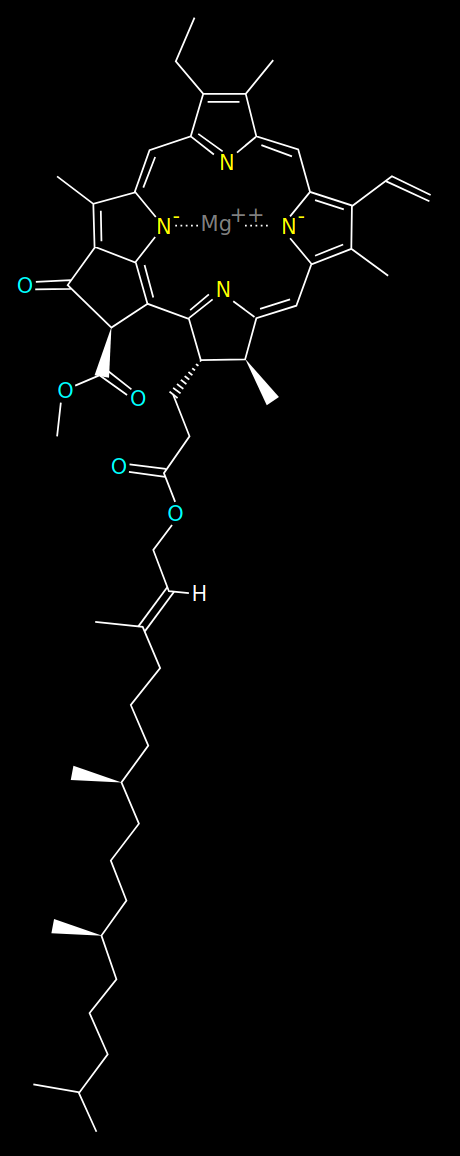
\includegraphics[width=0.8\textwidth]{chlorophyll.png}
%	\end{center}
%	\column{0.7\textwidth}
%	\normalsize
%	Biochemistry on Earth needs:
%
%\bigskip
%
%	\begin{itemize}
%		\item A way to make complicated structures
%		\item Something to dissolve them in so they can move around
%	\end{itemize}
%
%\bigskip
%\bigskip
%\bigskip
%
%Carbon is our ticket to complicated structure:
%
%	\begin{itemize}
%		\item It can form four bonds at once (4/8 valence electrons)
%		\item Carbon chains are the backbone of organic molecules
%	\end{itemize}
%
%	\bigskip
%
%Water is a good solvent:
%
%	\begin{itemize}
%		\item It is liquid at temperatures on Earth
%		\item It dissolves most things
%		\item It is made of very common atoms (hydrogen and oxygen)
%	\end{itemize}
%\end{columns}
%	}
%
%\frame{\frametitle{\textbf{Ask the Physicist: non-carbon-based life?}}
%\Large
%Could we replace these pieces?
%
%\pause
%
%\begin{columns}
%	\column{0.3\textwidth}
%	\begin{center}
%	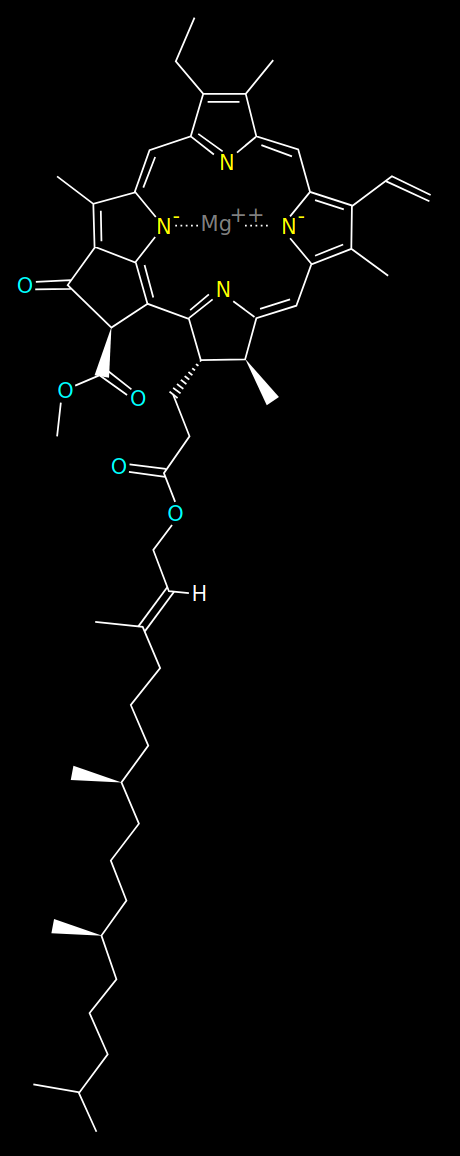
\includegraphics[width=0.8\textwidth]{chlorophyll.png}
%	\end{center}
%	\column{0.7\textwidth}
%	\normalsize
%
%	Other ``tetravalent'' (four-bond) atoms could also be the basis for structures: 
%
%	\begin{itemize}
%		\item Silicon and germanium are both also tetravalent 
%		\item Silicon is 1/10 as common as carbon and germanium is 1/200,000 as common
%		\item Complex carbon molecules have been observed in space...
%		\item ... but silicon ones haven't.
%	\end{itemize}
%
%	\bigskip
%
%There are other solvents:
%
%	\begin{itemize}
%		\item Ammonia is another possibility of an ionic solvent 
%		\item There are methane and ethane lakes on the surface of Titan
%	\end{itemize}
%
%Complex chemistry based on these would need very different temperatures and pressures than carbon/water life!
%\end{columns}
%	}
%

\frame{
\BC
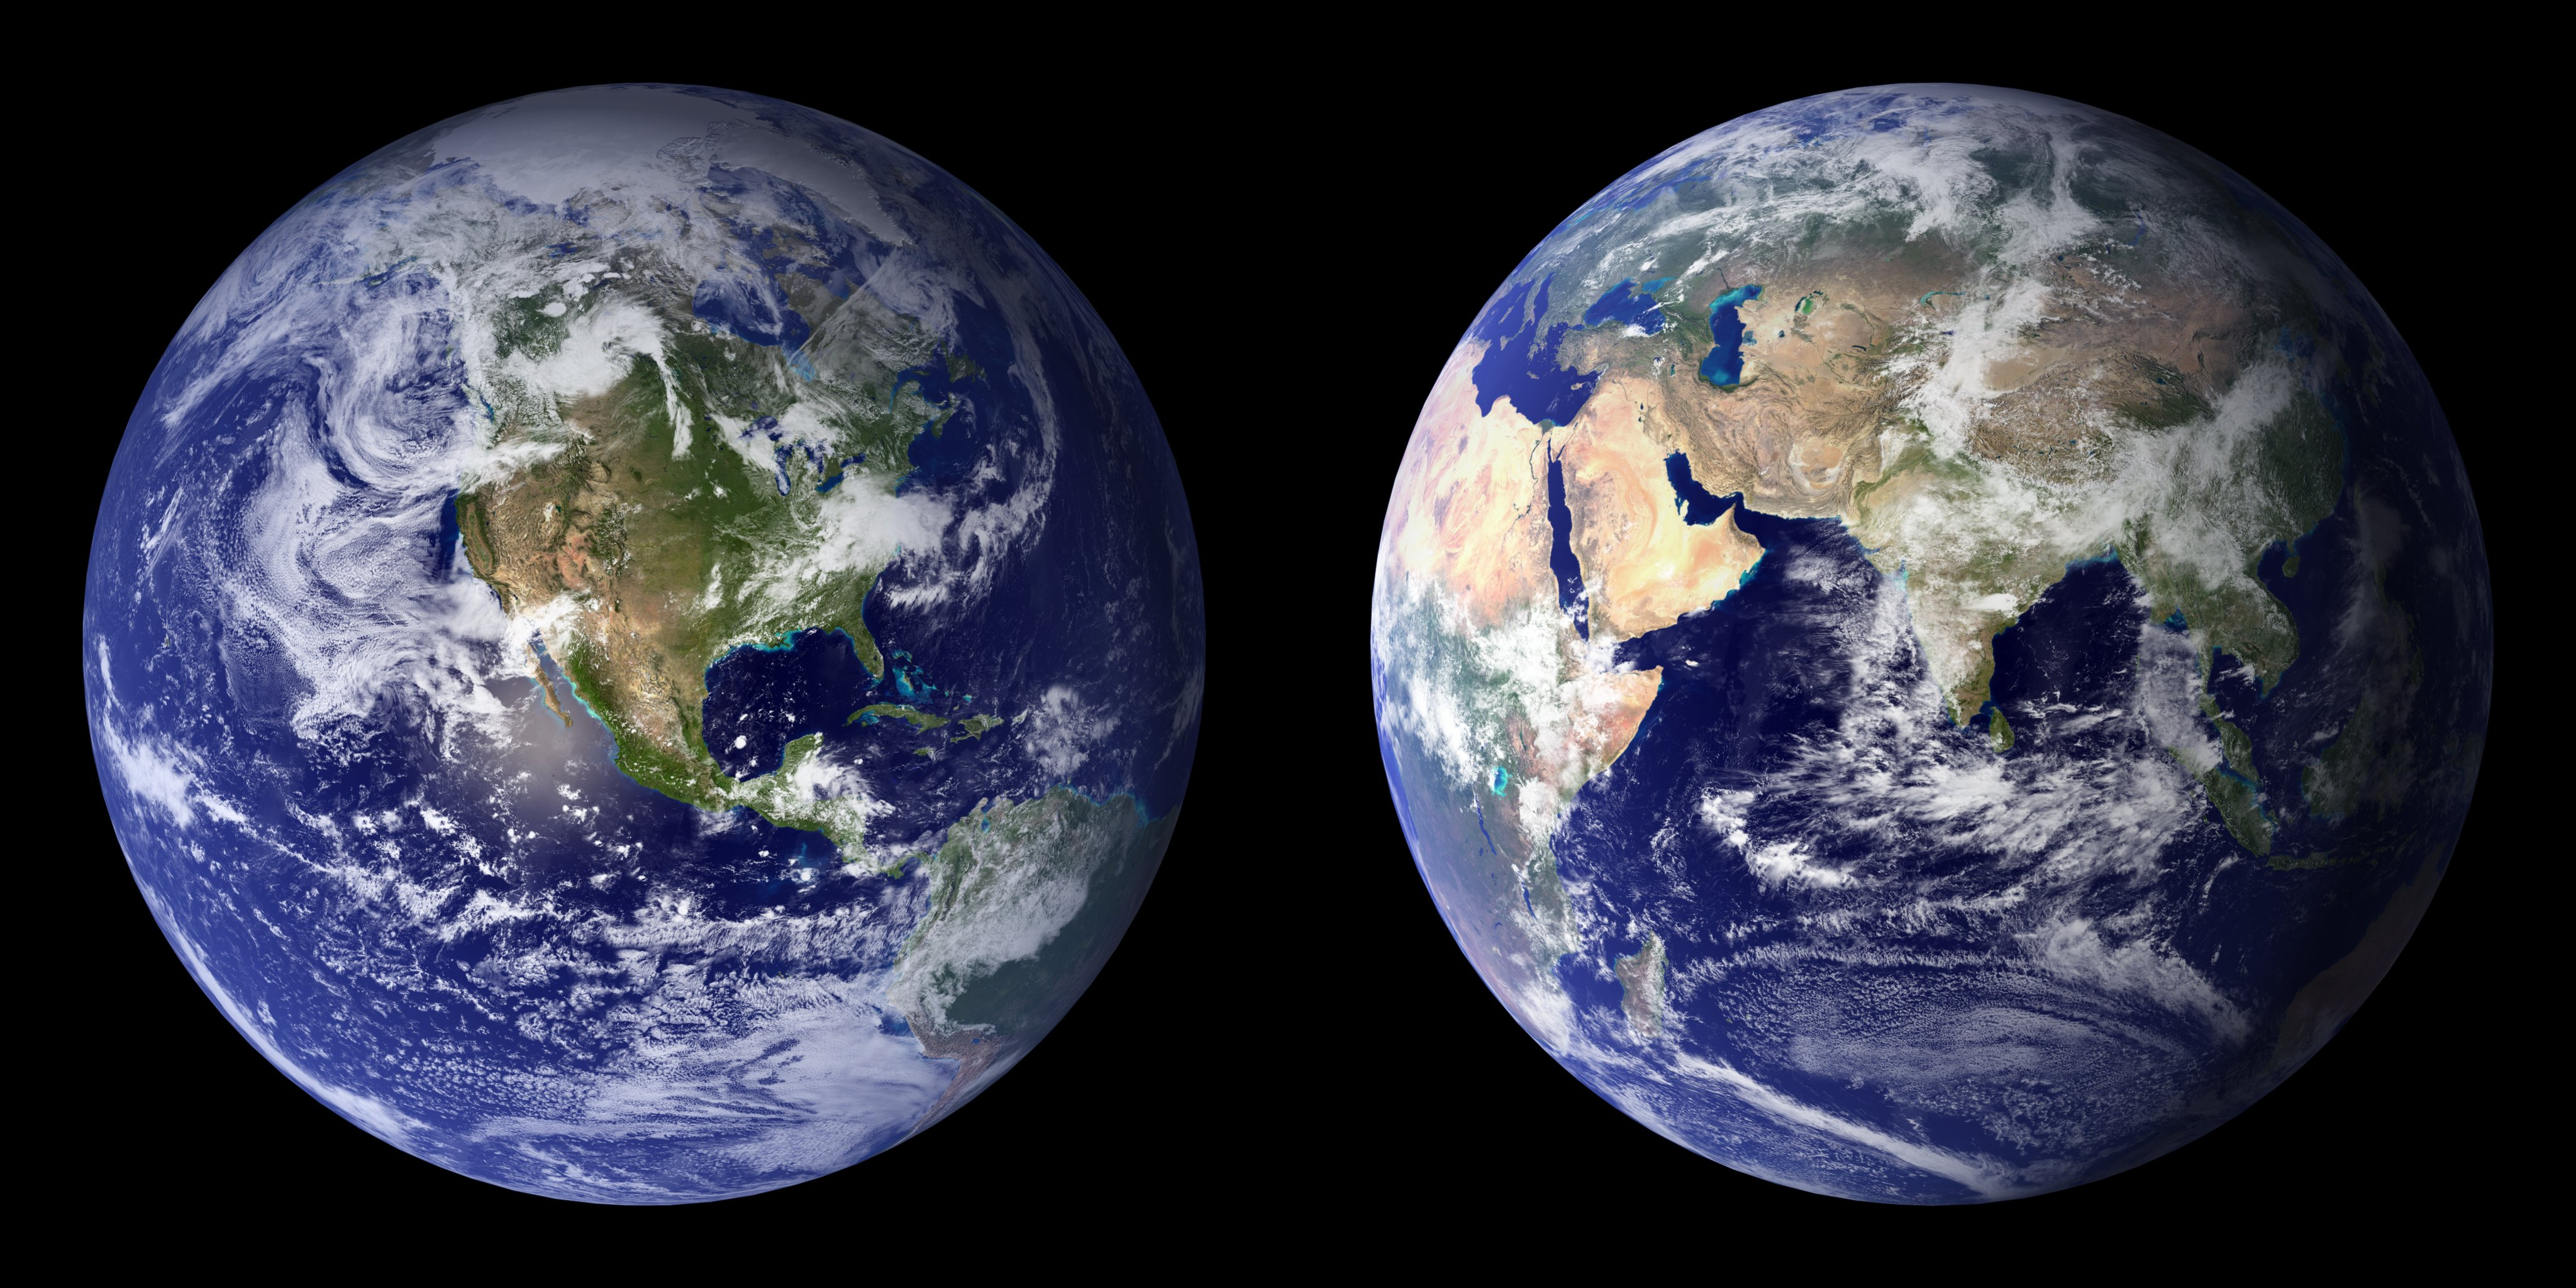
\includegraphics[width=\textwidth]{blue-marble.jpg}

\bigskip
\Large
What kind of world is this? What {\it can't} you see?
\EC
}


\frame{\frametitle{\textbf{Help sessions}}
\Large
Questions about the {\it Exercise-Tutorials?} Want to study with me? Come chat!

\bigskip
\bigskip
\bigskip

This is the absolute very best thing you can do to study for my class.

\bigskip
\bigskip

Come by the Clinic, Physics Building 112, and ask questions, or ask on Discord.

\bigskip

I also have office hours Wednesday 2-4 or Friday 9-11; come see me in room 215!
}


\frame{
\Large
Today: consequences of the Earth's {\bf revolution}:
\BI
\item{How is the Sun different from the other stars?}
\item{What's this zodiac business?}
\item{What does it mean for the Sun to be ``in Aries''?}
\pause
\item{We will see how this is only complicated because of {\bf how we keep time}}
\EI
}

\frame{\frametitle{\textbf{Which is true about the Sun?}}
\large
\color{A}A: The celestial sphere model predicts its motion exactly\\
\bigskip
\color{B}B: The celestial sphere model predicts its daily motion, but isn't accurate for longer times \\
\bigskip
\color{C}C: The celestial sphere model is completely wrong for the Sun
\bigskip
}

\frame{
\Large

Why is the celestial sphere model a bit wrong for the Sun?

\bigskip
\bigskip
\bigskip
\bigskip

\color{A}A: The Sun is close enough that the Earth's movement matters, unlike for other stars \\
\bigskip
\color{B}B: The Sun lies on a different celestial sphere than the stars, which turns at a different rate \\
\bigskip
\color{C}C: Angels push the Sun around on the celestial sphere, so it moves \\
\bigskip
\color{D}D: The Sun is close enough that we notice its movement, unlike the other stars
}




\frame{\frametitle{\textbf{A demonstration}}
\Large
Let's use {\it Stellarium} to revisit the same time every night -- say, midnight.

\pause\bigskip\bigskip

... What's wrong?

\pause\bigskip\bigskip

... isn't the celestial sphere supposed to rotate once per day?

... Why are the stars moving?

... What's wrong?

}


\frame{\frametitle{\textbf{A demonstration}}
\Large
Now let's look at the sky during the {\it daytime}, pretending the atmosphere is gone.

\bigskip
\bigskip
\bigskip

\pause

Which moves more, the sun or the stars?

\bigskip
\bigskip
\bigskip
\pause

\BI
\item{The Sun just moves up and down a little bit, and the stars spin!}
\item{... why is this?}
\EI
}

\frame{
\Huge
\BC Let's try to understand this on paper. \EC
}

\frame{
\Huge
\BC Work through the {\it Tutorial-Exercise} for today. Your next homework is
on the back; you can possibly finish it in class today. \EC

\bigskip
\BC \large We will talk about something else after this.
\EC
}



\frame{
\Large

\begin{columns}
\column{0.5\textwidth}
If the Earth is in the white position here, and the observer is the yellow dot (with the arrow sticking out of their head), what time is it?

\bigskip
\bigskip
\bigskip

\color{A}A: Noon \\
\color{B}B: Midnight \\
\color{C}C: Sunrise \\
\color{D}D: Sunset 
\column{0.5\textwidth}
\BC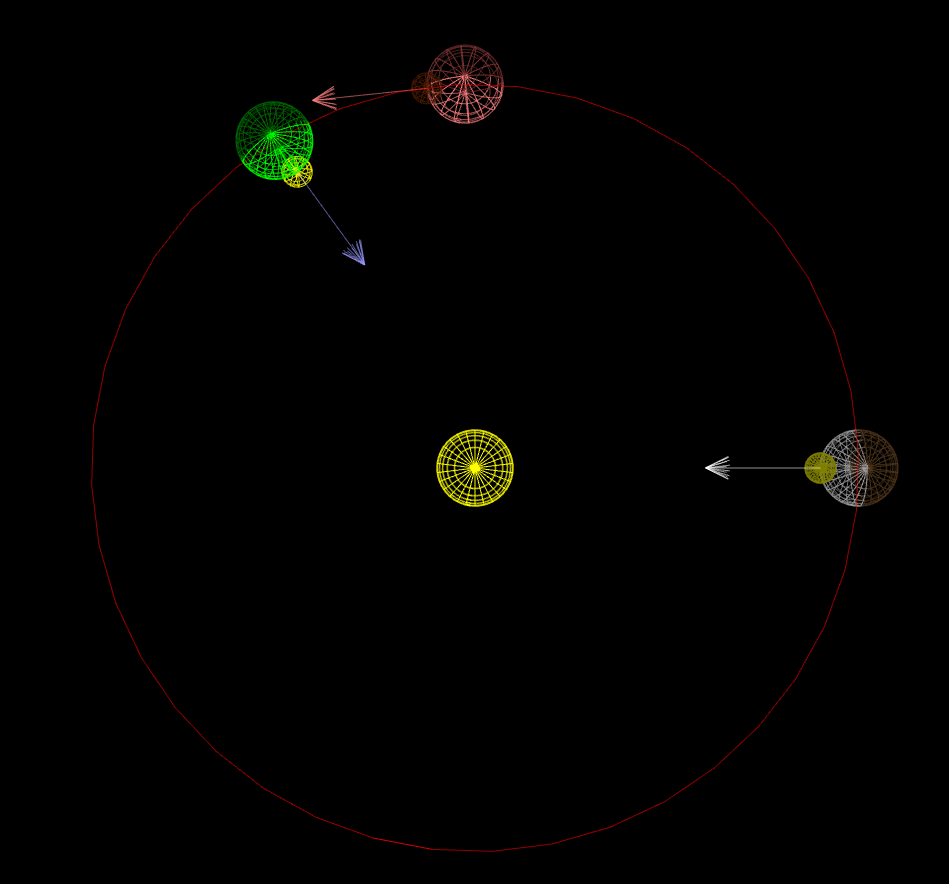
\includegraphics[width=0.9\textwidth]{day-question-1.png}\EC
\end{columns}

}

\frame{
\Large
\begin{columns}
\column{0.5\textwidth}
Which image shows the position of the Earth {\it \bf exactly} one day later?
\column{0.5\textwidth}
\BC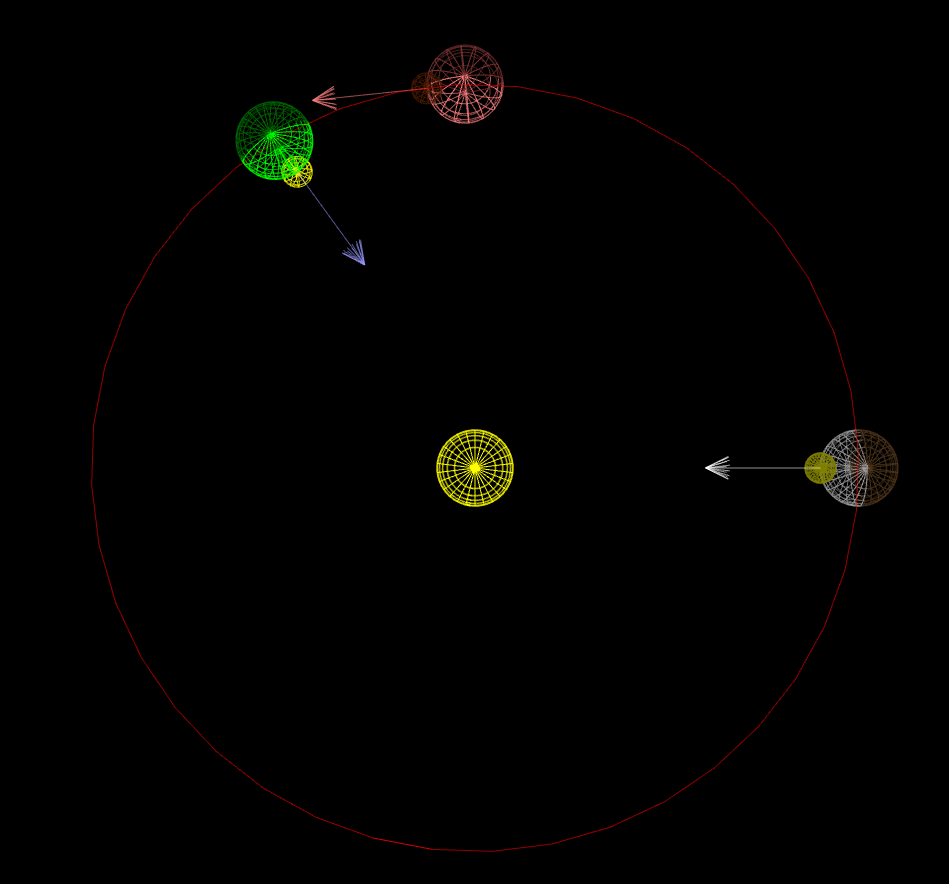
\includegraphics[width=0.9\textwidth]{day-question-1.png}\EC
\end{columns}

\bigskip
\bigskip

\color{A}A: The red one \\
\color{B}B: The green one \\
\pause
\color{C}C: Depends on what you mean by ``a day'' \\
\pause
\color{D}D: The Earth moves? BURN THE HERETIC!

}


\frame{
\Large
There are {\it two kinds} of day!

\BI
\item{Solar day: judged by the position of the Sun}
\item{Sidereal day (sih-dee-ree-al): judged only by the rotation of the Earth with respect to the stars}
\EI
}

%\frame{
%
%\BC\Huge Work through the {\it Lecture Tutorials}, pp. 11-12.
%
%\bigskip
%
%\large
%We will talk about something else after this.
%\EC
%}
%
%\frame{\frametitle{\textbf{Two kinds of day!}}
%\Large
%
%\BC Demo in {\it Stellarium:} \EC
%
%\bigskip
%\bigskip
%\begin{columns}
%\column{0.5\textwidth}
%\Large
%In one solar day...
%\column{0.5\textwidth}
%\Large
%In one sidereal day...
%\end{columns}
%\begin{columns}
%\column{0.5\textwidth}
%\BI
%\large
%\item{The stars move a lot}
%\item{...since the Earth isn't pointed in the same direction}
%\item{The Sun moves higher or lower in the sky a little bit}
%\item{Exactly 24h}
%\EI
%
%\column{0.5\textwidth}
%\BI
%\large
%\item{The stars don't move at all}
%\item{... since the Earth is pointed in the same direction}
%\item{The Sun moves a lot, since the Earth has moved}
%\item{A little bit less than 24h}
%\EI
%\end{columns}
%}
%
%\frame{\frametitle{Lecture tutorials, again}
%\Huge
%\BC
%Complete pp. 12-16.
%\EC
%
%\large
%\bigskip
%If you don't have time to finish, that's okay. Finishing this is great practice at home, though!
%}


\end{document}
